% Copyright 2021 Fausto Spoto
%
% Licensed under the Apache License, Version 2.0 (the "License");
% you may not use this file except in compliance with the License.
% You may obtain a copy of the License at
%
%    http://www.apache.org/licenses/LICENSE-2.0
%
% Unless required by applicable law or agreed to in writing, software
% distributed under the License is distributed on an "AS IS" BASIS,
% WITHOUT WARRANTIES OR CONDITIONS OF ANY KIND, either express or implied.
% See the License for the specific language governing permissions and
% limitations under the License.

\documentclass[11pt]{beamer}  %% versione proiettore
%%\documentclass[11pt,handout]{beamer} %% versione stampa
\usepackage{slides}

\usepackage{relsize}

\mode<article>
{
  \usepackage{fullpage}
  \usepackage{hyperref}
}

\mode<presentation>
{
  \setbeamertemplate{background canvas}[vertical shading][bottom=red!10,top=blue!10]
  \usetheme{Course}
  \usefonttheme[onlysmall]{structurebold}
}

\subtitle{Laboratorio di co-design}
\title{Veneto Smart Region}
\institute{Universit\`a di Verona}
\date{Maggio 2021}

\setbeamercovered{invisible}

\def\codesize{\smaller}
\def\<#1>{\codeid{#1}}
\newcommand{\codeid}[1]{\ifmmode{\mbox{\codesize\ttfamily{#1}}}\else{\codesize\ttfamily #1}\fi}

\hypersetup{
  colorlinks=false,
%  linkcolor=blue!50!red,
%  urlcolor=blue!70!black,
  linkbordercolor=red,% hyperlink borders will be red
  pdfborderstyle={/S/U/W 1}% border style will be underline of width 1pt
}

\begin{document}

\begin{frame}
  \titlepage
\end{frame}

\begin{frame}\frametitle{Blockchain e smart city/region/nation}

  \begin{itemize}
  \item \href{https://www.am.pictet/it/blog/articoli/tecnologia-e-innovazione/la-blockchain-al-servizio-delle-smart-city}{La blockchain al servizio delle smart city} (2018)
  \item \href{https://www.iberdrola.com/innovation/blockchain-for-smart-cities-urban-management}{La blockchain al servizio della gestione urbana} (2018)
  \item \href{https://www.weforum.org/agenda/2021/04/how-blockchain-can-empower-smart-cities-gtgs21}{Come la blockchain accender\`a le smart city} (2021)
  \end{itemize}

  \bigskip  
  \begin{itemize}
  \item \emph{maggiore trasparenza delle procedure amministrative}
  \item \emph{comunicazione diretta con i cittadini}
  \item \emph{integrit\`a delle informazioni}
  \item \emph{certificazione di efficienza dei processi gestionali}
  \item \emph{gestione energetica efficiente}
  \item \emph{gestione efficiente del trasporto pubblico}
  \item \emph{certificazione delle filiari produttive}
  \item \emph{ottimizzazione della raccolta dei rifiuti}
  \item \emph{consultazioni pubbliche sicure}
  \item \emph{convergenza con IoT}
  \end{itemize}

\end{frame}

\begin{frame}\frametitle{Il ciclo delle aspettative}

  \begin{center}
    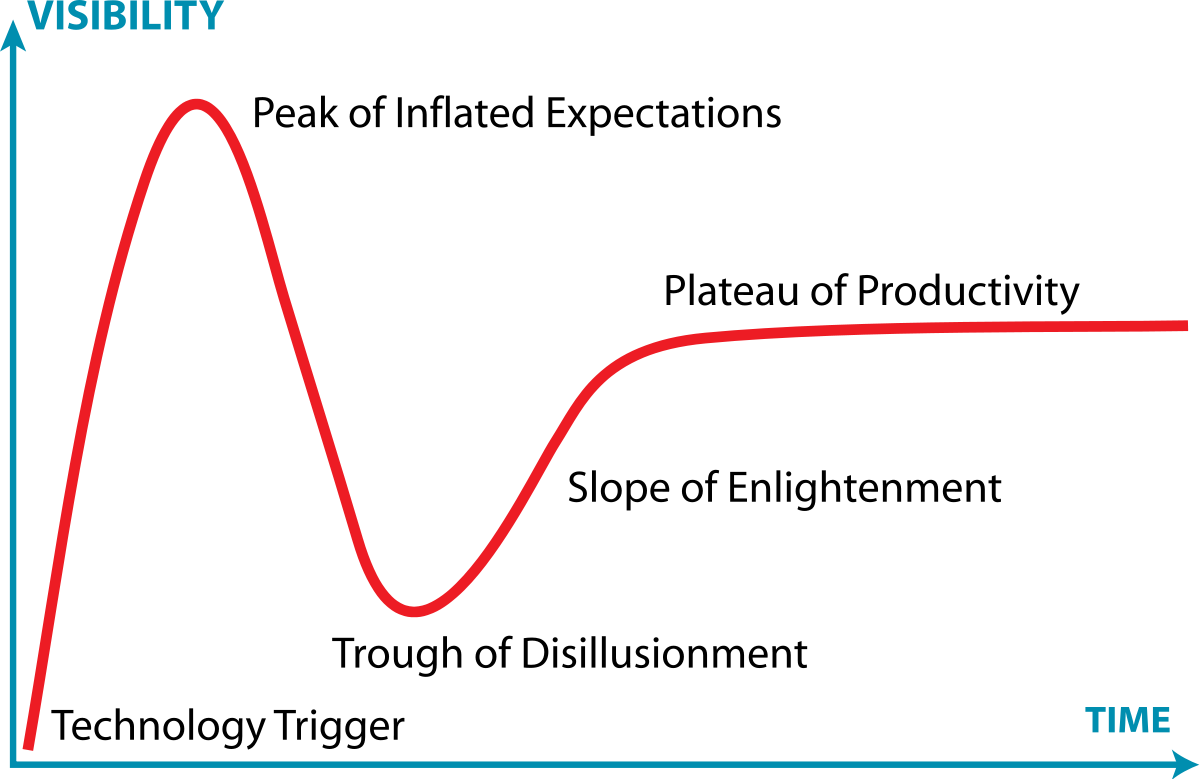
\includegraphics[width=\textwidth,clip=false]{pictures/hype-cycle.png}
  \end{center}

\end{frame}

\begin{frame}\frametitle{Serve una blockchain? Quale?}

  Una blockchain \`e un valore aggiunto quando:
  \begin{enumerate}
  \item i dati sono importanti
  \item manca la fiducia reciproca fra i partner
  \item la sua governance \`e \emph{sufficientemente} aperta e indipendente
  \end{enumerate}

  \medskip

  \begin{center}
    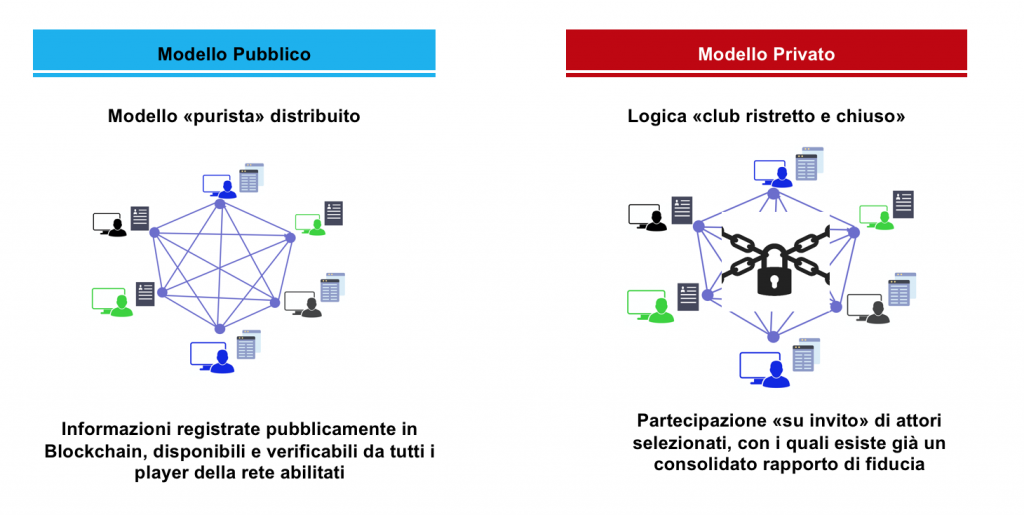
\includegraphics[width=10.5cm,clip=false]{pictures/blockchain-private-e-pubbliche.png}
  \end{center}

\end{frame}

\begin{frame}\frametitle{Cosa vuol dire \emph{sufficientemente} aperta e indipendente?}

  Sicuramente non significa questo:
  \begin{center}
    \href{https://www.coindesk.com/china-to-create-it-can-control}{Lo sforzo della Cina per una blockchain controllata} (2021)
  \end{center}

  \medskip

  \begin{center}
    {\color{red}\emph{Una blockchain privata con nodi validatori gestiti da poche amministrazioni pubbliche appartenenti a una smart region
    \underline{non} pu\`o essere considerata aperta e indipendente}}
  \end{center}

  \medskip

  \begin{center}
    {\color{blue}{Si potrebbe immaginare una blockchain a livello europeo, con regole di ingresso e selezione di nodi validatori applicabili
    sia a societ\`a private che ad amministrazioni pubbliche degli Stati membri, con meccanismi premiali e di rotazione imposti da smart contract}}
  \end{center}

  \medskip

  \begin{center}
    Esiste il tasto OFF ?
  \end{center}
  
\end{frame}

\begin{frame}\frametitle{Aspettative realistiche}

  \begin{center}
    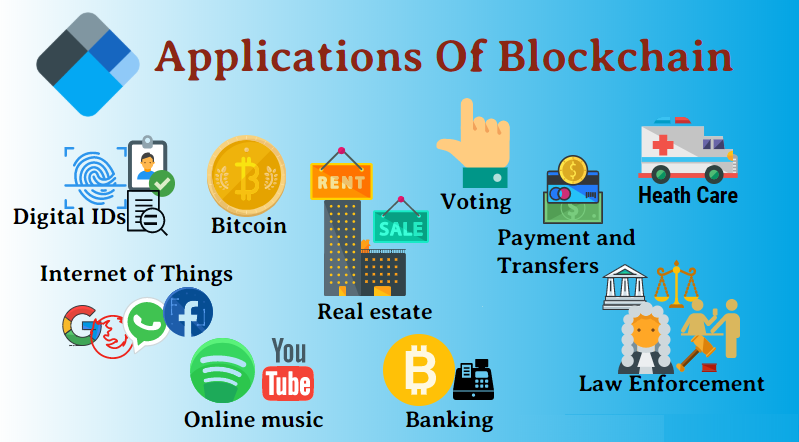
\includegraphics[scale=0.4,clip=false]{pictures/blockchain-applications.png}
  \end{center}

  \begin{center}
    Molte di queste attivit\`a sono legate alla pubblica amministrazione!
  \end{center}
  
\end{frame}

\end{document}
